\documentclass[]{article}
\usepackage{lmodern}
\usepackage{amssymb,amsmath}
\usepackage{ifxetex,ifluatex}
\usepackage{fixltx2e} % provides \textsubscript
\ifnum 0\ifxetex 1\fi\ifluatex 1\fi=0 % if pdftex
  \usepackage[T1]{fontenc}
  \usepackage[utf8]{inputenc}
\else % if luatex or xelatex
  \ifxetex
    \usepackage{mathspec}
  \else
    \usepackage{fontspec}
  \fi
  \defaultfontfeatures{Ligatures=TeX,Scale=MatchLowercase}
\fi
% use upquote if available, for straight quotes in verbatim environments
\IfFileExists{upquote.sty}{\usepackage{upquote}}{}
% use microtype if available
\IfFileExists{microtype.sty}{%
\usepackage{microtype}
\UseMicrotypeSet[protrusion]{basicmath} % disable protrusion for tt fonts
}{}
\usepackage{hyperref}
\hypersetup{unicode=true,
            pdftitle={Assignment 1 - Report},
            pdfauthor={Pietro Alovisi},
            pdfborder={0 0 0},
            breaklinks=true}
\urlstyle{same}  % don't use monospace font for urls
\usepackage{graphicx,grffile}
\makeatletter
\def\maxwidth{\ifdim\Gin@nat@width>\linewidth\linewidth\else\Gin@nat@width\fi}
\def\maxheight{\ifdim\Gin@nat@height>\textheight\textheight\else\Gin@nat@height\fi}
\makeatother
% Scale images if necessary, so that they will not overflow the page
% margins by default, and it is still possible to overwrite the defaults
% using explicit options in \includegraphics[width, height, ...]{}
\setkeys{Gin}{width=\maxwidth,height=\maxheight,keepaspectratio}
\IfFileExists{parskip.sty}{%
\usepackage{parskip}
}{% else
\setlength{\parindent}{0pt}
\setlength{\parskip}{6pt plus 2pt minus 1pt}
}
\setlength{\emergencystretch}{3em}  % prevent overfull lines
\providecommand{\tightlist}{%
  \setlength{\itemsep}{0pt}\setlength{\parskip}{0pt}}
\setcounter{secnumdepth}{0}
% Redefines (sub)paragraphs to behave more like sections
\ifx\paragraph\undefined\else
\let\oldparagraph\paragraph
\renewcommand{\paragraph}[1]{\oldparagraph{#1}\mbox{}}
\fi
\ifx\subparagraph\undefined\else
\let\oldsubparagraph\subparagraph
\renewcommand{\subparagraph}[1]{\oldsubparagraph{#1}\mbox{}}
\fi

\title{Assignment 1 - Report}
\author{Pietro Alovisi}
\date{}

\begin{document}
\maketitle

\section{The Implementation}\label{the-implementation}

The implementation is done in Matlab, following the suggested project
structure.

I achieved good computational performance by using vectorized
operations. In particular

\section{Results}\label{results}

\subsection{test 1}\label{test-1}

\begin{figure}[h]
\centering
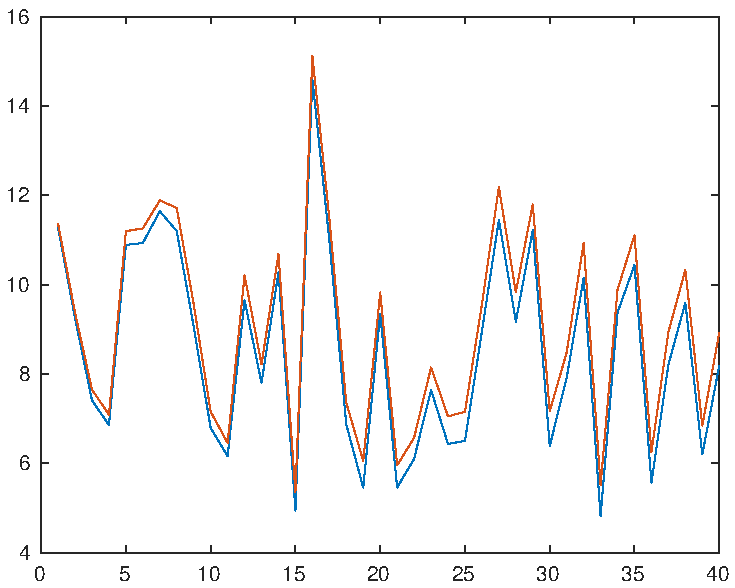
\includegraphics{../Result_Pics/b100e40eta1la0.pdf}
\caption{This is the caption}
\end{figure}

\begin{figure}[h]
\centering
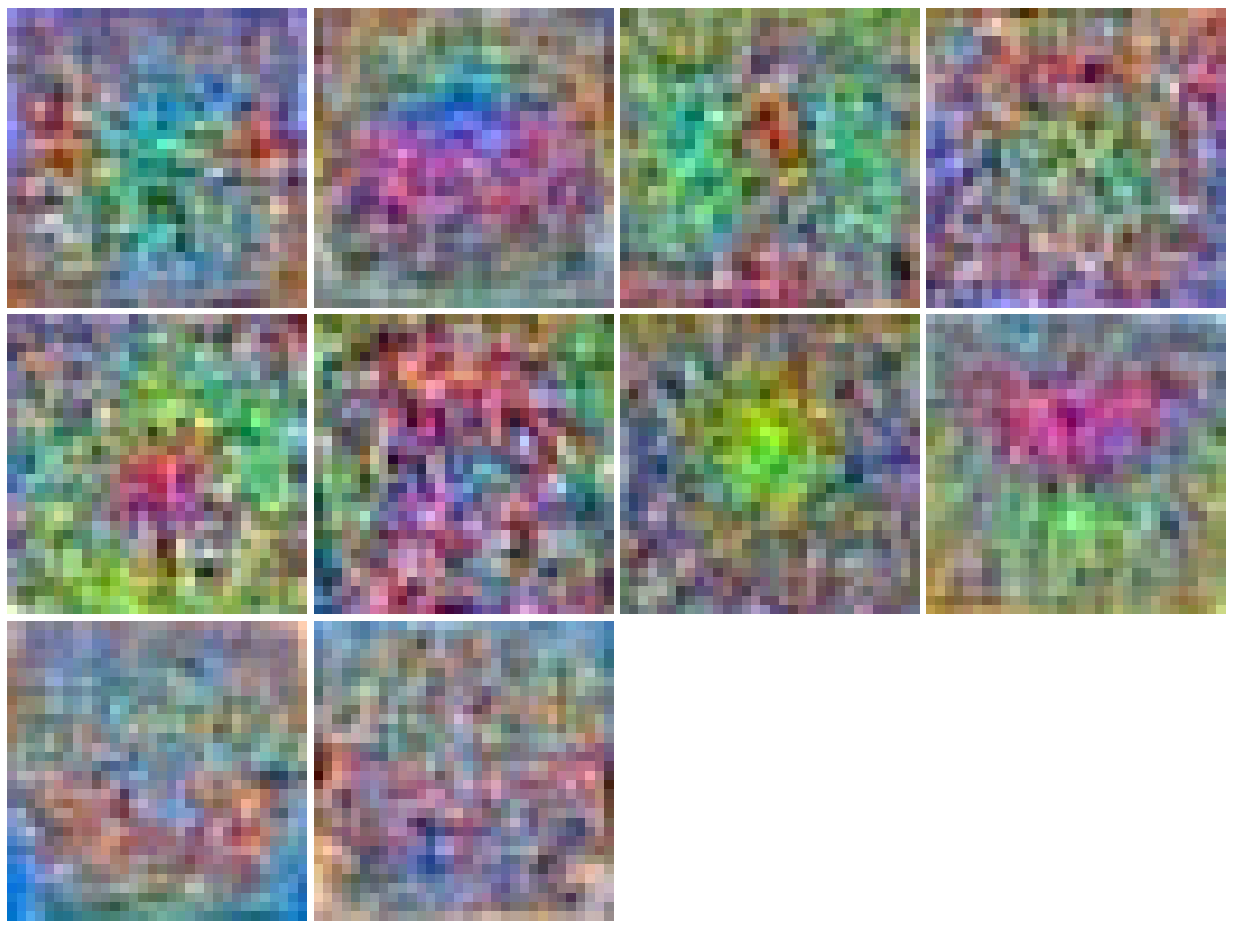
\includegraphics{../Result_Pics/b100e40eta1la0proto.pdf}
\caption{This is the caption}
\end{figure}

lambda = 0.0;

GDparams.n\_batch = 100; GDparams.eta = 0.1; GDparams.n\_epochs = 40;

23.1 acc with high variance (as low as 19 as high as 28) \#\# test 2

\begin{figure}[h]
\centering
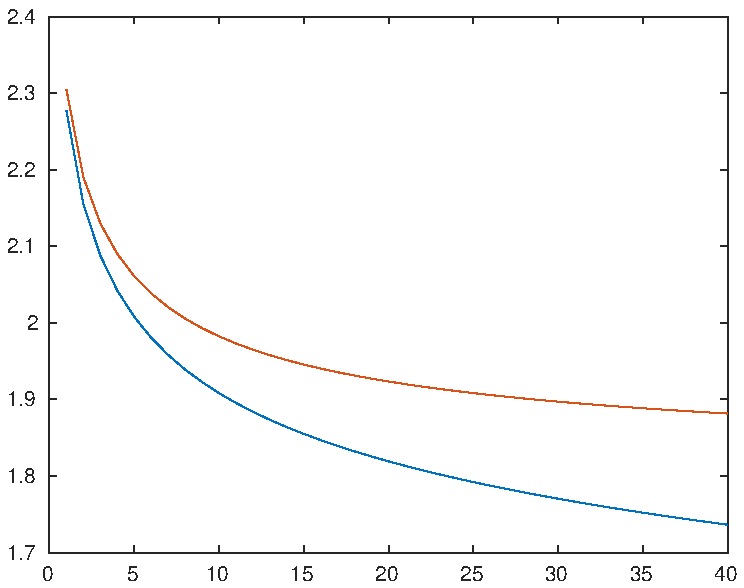
\includegraphics{../Result_Pics/b100e40eta01la0.pdf}
\caption{This is the caption}
\end{figure}

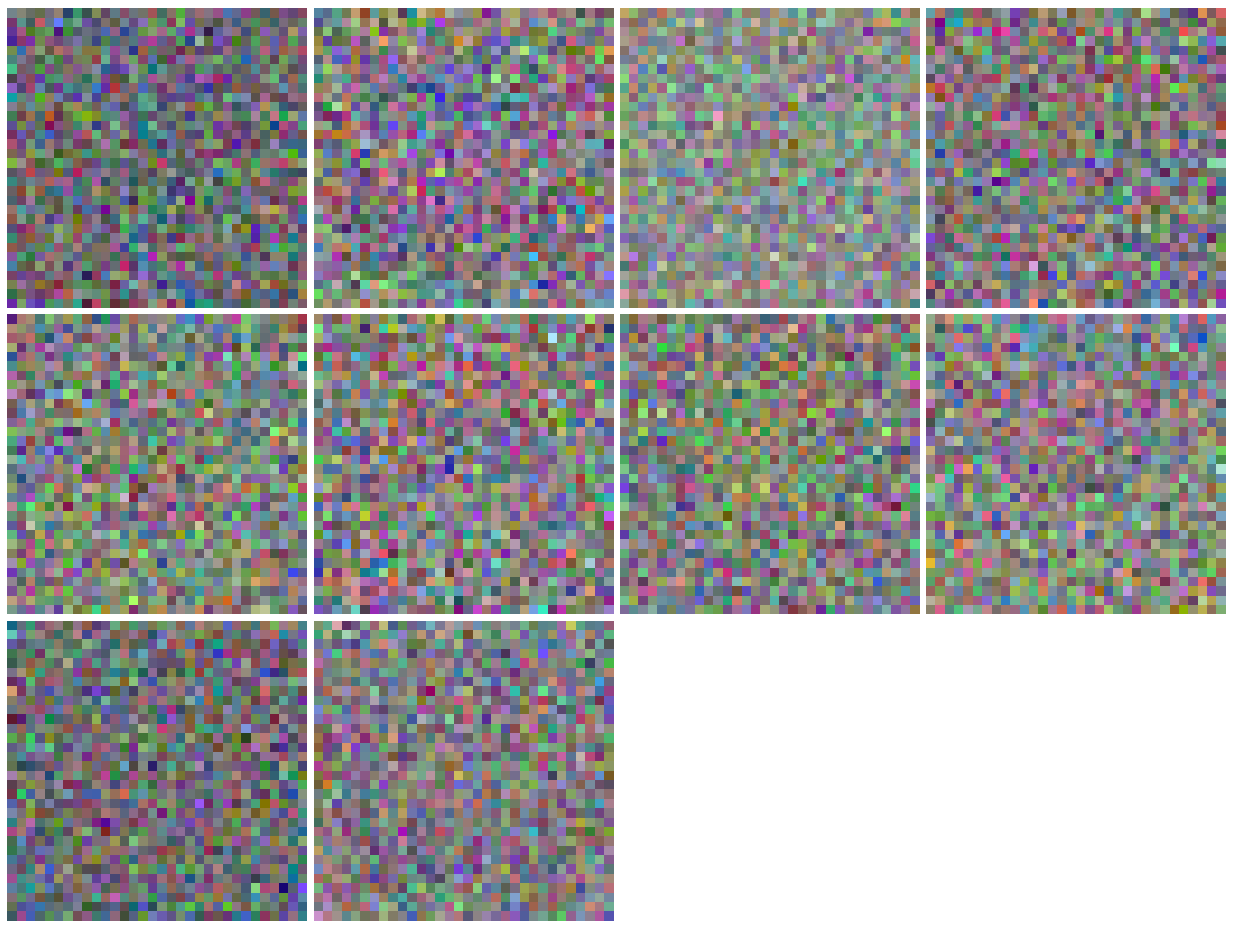
\includegraphics{../Result_Pics/b100e40eta01la0proto.pdf} lambda = 0.0;

GDparams.n\_batch = 100; GDparams.eta = 0.01; GDparams.n\_epochs = 40;

34,5 acc steady

\subsection{test 3}\label{test-3}

\begin{figure}[h]
\centering
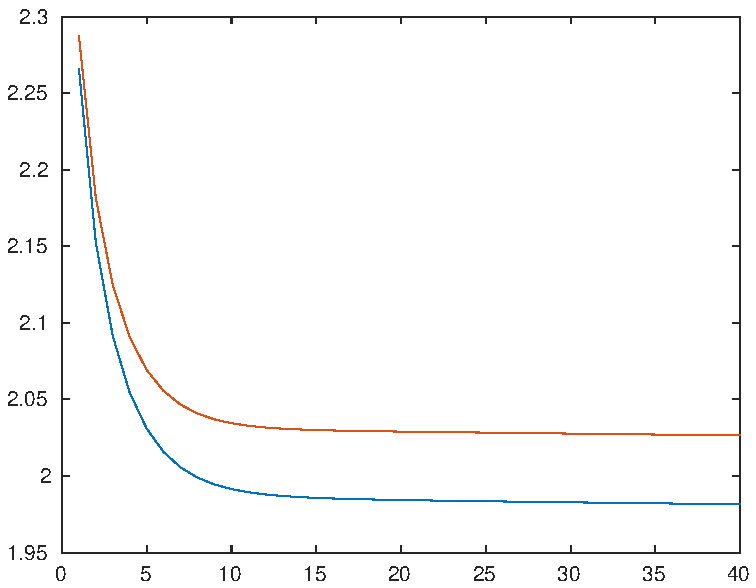
\includegraphics{../Result_Pics/b100e40eta01la_1.pdf}
\caption{This is the caption}
\end{figure}

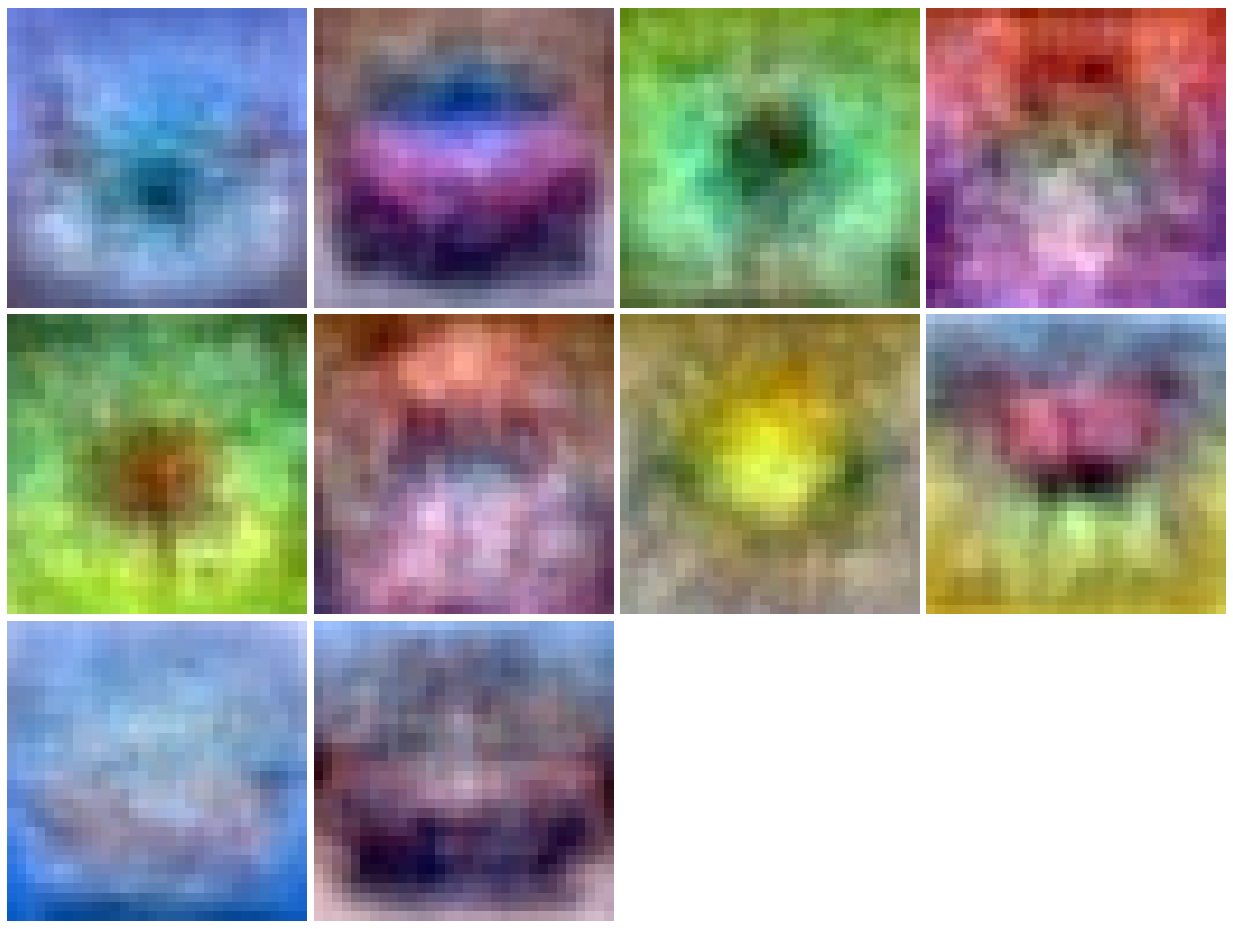
\includegraphics{../Result_Pics/b100e40eta01la_1proto.pdf} lambda = 0.1;

GDparams.n\_batch = 100; GDparams.eta = 0.01; GDparams.n\_epochs = 40;

34,3 acc steady, std\_dev less than 1\%

\subsection{test 4}\label{test-4}

\begin{figure}[h]
\centering
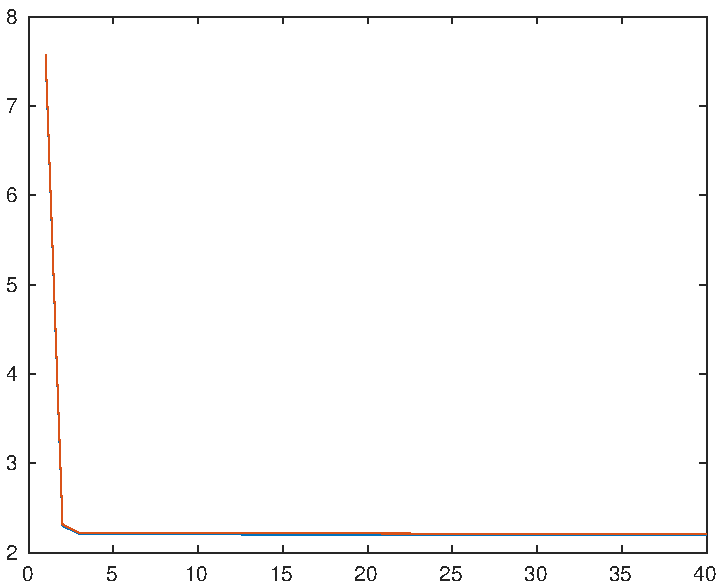
\includegraphics{../Result_Pics/b100e40eta01la1_.pdf}
\caption{This is the caption}
\end{figure}

\begin{figure}[h]
\centering
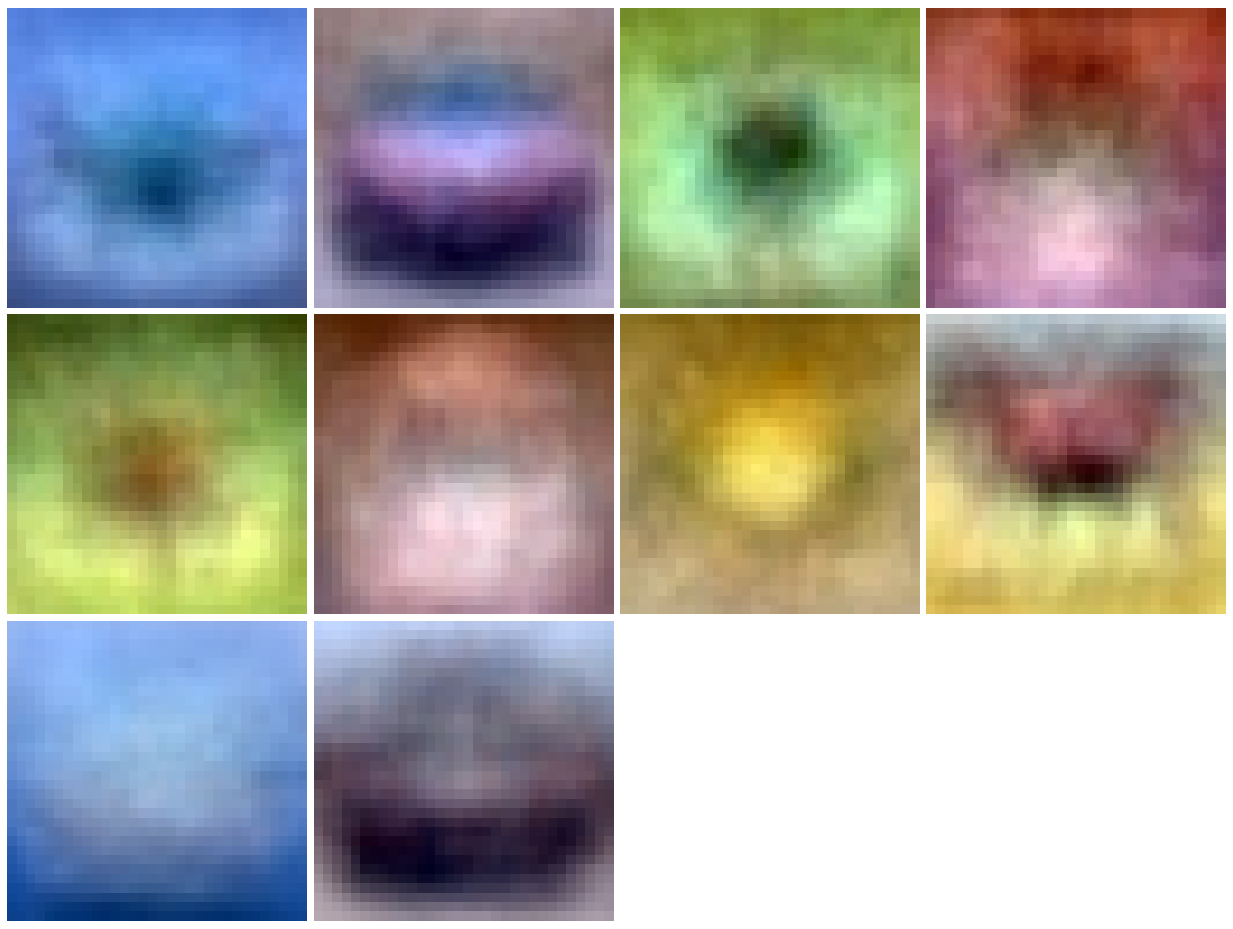
\includegraphics{../Result_Pics/b100e40eta01la1_proto.pdf}
\caption{This is the caption}
\end{figure}

lambda = 1.0;

GDparams.n\_batch = 100; GDparams.eta = 0.01; GDparams.n\_epochs = 40;

21,5 acc steady, std\_dev less than 1\%

\end{document}
